\subsection{Система тонких клиентов}
Тонкий клиент, как и классический терминал 50–60-х годов, дает пользователю возможность
взаимодействия с удаленным компьютером. Разница в том, что если мощностей терминалов,
мэйнфреймов и пропускной способности сети хватало только для отправки текстовых команд и
получения текстовых результатов, то современные тонкие клиенты позволяют пользователям
взаимодействовать и с графическими интерефейсами, работать с графикой и даже
воспроизводить видео. Для пользователя тонкого клиента взаимодействие с удаленным
рабочим столом должно выглядеть неотличимо от обычного ПК. Современные ТК позволяют это
сделать.

Система, основанная на тонких клиентах, состоит из терминального сервера и одного и
более ТК. На терминальном сервере установлена ОС, позволяющая подключение ТК. Все
клиенты настроены на подключение к этому серверу и занимаются только вводом-выводом
информации для взаимодействия с пользователем, и выполнением протоколов удаленного
доступа. Все вычисления, работа ОС и процессов, взаимодействие с устройствами хранения
информации выполняются на сервере. 

Таким образом, все ресурсоемкие процессы в системе ТК перенесены на сервер. Это
означает, что для клиентских машин нужно минимальное аппаратное обеспечение, достаточное
для вывода изображения на экран, работы с сетью и устройствами ввода-вывода. В качестве
таких клиентов могут выступать как специализированные устройства, так и устаревшие ПК,
мощности которых уже не хватает для привычных пользователям задач.
(см. рисунок~\ref{pic:PCtoTC}).

\begin{figure}[htpb]
    \center
    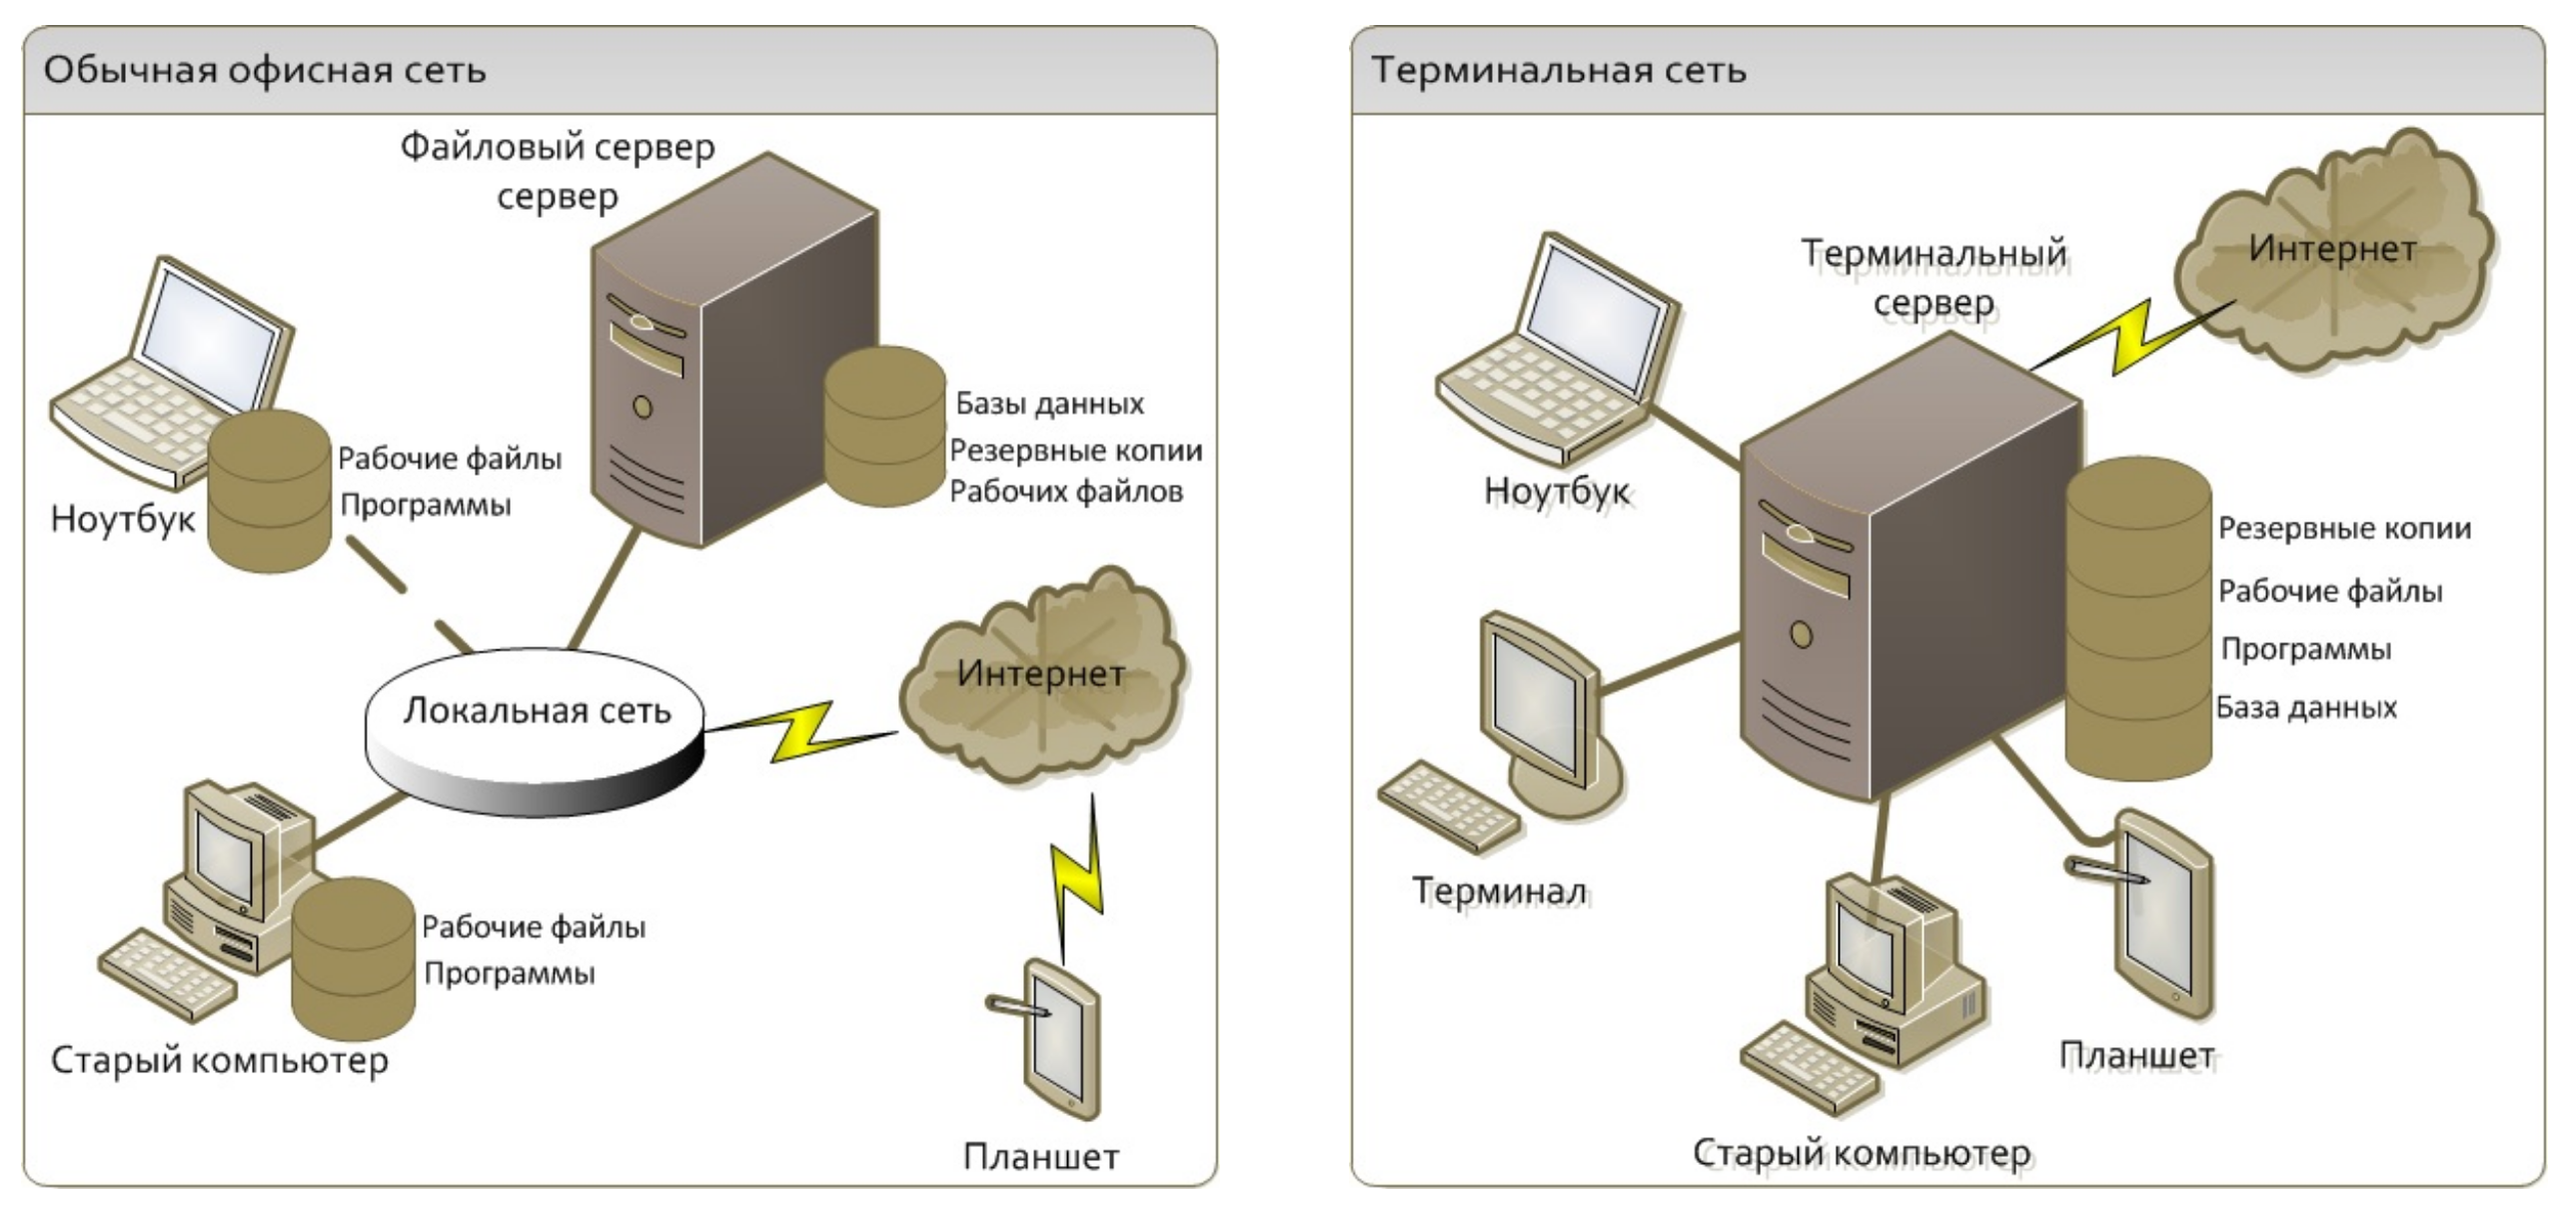
\includegraphics[width=\linewidth]{PCtoTC}
    \caption{Сравнение типовой и терминальной сетей. Источник: \cite{PCtoTCsrc}}
    \label{pic:PCtoTC}
\end{figure}

Преимущества систем, построенных на базе тонких клиентов:
\begin{itemize}
    \item   Экономия средств. Необходимость в постоянной модернизации всего парка
        компьютеров с выходом более новых и ресурсоёмких ОС и приложений исчезает.
        Модернизировать, при необходимости, нужно будет только терминальный сервер и
        серверы БД; терминалы не нуждаются в модернизации в течение длительного времени
        (7-10 лет). Лицензия терминального доступа стоит дешевле настольной ОС, не нужны
        локальные антивирусы, сложное ПО управления парком ПК, что значительно сокращает
        затраты. Снижается количество рутинных операций, а также перемещений IT
        персонала для обслуживания подразделений. При использовании терминала нет
        необходимости дополнительно приобретать источник бесперебойного питания для
        защиты от внезапного отключения питания, вся информация остается доступной на
        серверах. Даже при аппаратной замене ТК пользователь может продолжить работу.
    \item   Надежность. Использование серверной операционной системы и аппаратуры
        сервера повышает надежность работы и хранения данных. Выход из строя терминала,
        его утрата не повлекут за собой потерю или порчу данных на сервере.
    \item   Безопасность. Отсутствие на клиентских машинах жестких дисков, дисководов и
        приводов оптических дисков позволяет избежать несанкционированного копирования и
        выноса данных. Отсутствие непосредственной передачи данных по сети позволяет
        избежать их перехвата. Все программное обеспечение ставится только системным
        администратором. При краже или изъятии обычного компьютера есть риск потерять
        важные конфиденциальные данные, хранящиеся на нем. Терминал гораздо менее
        привлекателен для воров, т.к. не применим в домашних условиях, а при
        использовании тонких клиентов данные на конечном устройстве не хранятся.
    \item   Централизация. Все данные хранятся только на серверах, что упрощает
        процедуру резервного копирования, контроля версий ПО, контроля доступа
        пользователей. Всё ПО находится на серверах - это упрощает администрирование.
        Конечный пользователь не может повлиять на стабильность такой системы.
    \item   Эффективность. Загрузка процессора на ПК в большинстве случаев не превышает
        4-5\%. Терминальная система позволяет максимально полезно использовать
        вычислительные ресурсы сервера, распределяя их между работающими в данный момент
        пользователями.
    \item   Снижение энергопотребления. Тонкие клиенты используют
        энергоэффективные процессоры и не имеют подвижных компонентов, потребляют всего
        около 10\% мощности обычного ПК.
    \item   Тихая работа. Из-за низкого энергопотребления тепловыделение процессоров ТК
        невелико. Это позволяет использовать активные систмы охлаждения с малыми
        скоростями вращения вентиляторов, или использовать полностью пассивные системы
        охлаждения, что обеспечивает бесшумную работу клиентов.
    \item   Быстрое развертывание и обновление приложений. При использовании ТК вы
        просто устанавливаете новое ПО на серверах, и оно становится доступным сотням
        пользователей сразу после публикации.
    \item   Устранение поддержки конечных узлов. ПК – источник аппаратных проблем и
        проблем локальных конфигураций. При использовании ТК отпадает необходимость
        подходить к пользовательским устройствам для настройки системы, установки и
        ремонта программ, помощи в настройке приложений, замены сломанных деталей. ТК
        используют операционную систему терминального сервера, а приложения
        устанавливаются на серверах. Служба техподдержки может помогать пользователям
        посредством удаленного управления их терминальными сеансами. При выходе ТК из
        строя его легко заменить, что может выполнить специально назначенный сотрудник,
        даже не имеющий IT образования.
    \item   Защита от вирусов. Тонкие клиенты не подвержены заражению вирусами, на них
        антивирусное ПО не устанавливается. Достаточно установить антивирусное ПО на
        серверы компании. Локальный ПК не защищен от заражения при сбое параметров
        обновления или настройки антивируса и дальнейшего распространения вируса в ИС.
\end{itemize}

Из существенных недостатков системы на базе ТК можно выделить только необходимость
первоначальной настройки системы. Для внедрения данной системы нужно подготовить
достаточно производительный терминальный сервер, а также настроить его в соответствии с
планируемой архитектурой сети.  Также для корректной работы всей сети администратор
должен знать о ее организации.  Требуется более высокая квалификация администратора,
т.к. в его обязанности также будет входить поддержка протоколов удаленного доступа,
использованных в системе.  Однако, это компенсируется более низкой требуемой
квалификацией техников.
